\documentclass[11pt, a4paper]{article}
\usepackage[utf8]{inputenc}
\usepackage[T1]{fontenc}
\usepackage[french]{babel}
\usepackage{graphicx}
\usepackage{geometry}
\usepackage{hyperref}
\usepackage{booktabs}
\usepackage{xcolor}

\geometry{a4paper, margin=2.5cm}

\title{\textbf{Synthèse des Expérimentations NLI} \\ \Large{Comparaison des méthodes PEFT (IA$^3$ vs LoRA) en conditions Few-Shot}}
\author{Projet TER M1 -- Rapport d'expérimentation}
\date{\today}

\begin{document}

\maketitle

\section{Contexte : Full-Data vs Few-Shot en NLI}
Le cadre de ce projet de TER vise à évaluer la capacité des modèles de langage pré-entraînés (CamemBERT, FlauBERT) à résoudre des tâches d'inférence en langage naturel (NLI) en français.
Nous avons commencé par définir la borne supérieure des performances (\textit{Full-Data Fine-Tuning}) : avec accès à la totalité d'un dataset (plus de 50 000 exemples), un modèle CamemBERT atteint entre 65\% et 85\% d'exactitude.

Toutefois, la disponibilité de milliers de données annotées est rare en entreprise. L'objectif de notre phase d'expérimentation croisée est d'étudier l'effondrement des performances en condition de privation de données (\textit{Extreme Few-Shot}, soit entre 8 et 128 exemples).

\section{Approche Technique : Comparaison LoRA et IA$^3$}
Pour éviter l'oubli catastrophique et le sur-apprentissage immédiat qui se produisent lorsqu'on fine-tune un modèle entier sur 8 exemples, nous avons utilisé des méthodes de fine-tuning efficaces en paramètres (PEFT).
Nous avons implémenté et comparé deux architectures :
\begin{itemize}
    \item \textbf{LoRA} : Injection de matrices de bas rang. Bien qu'efficiente, elle modifie environ $\sim 1.06\%$ des poids du modèle.
    \item \textbf{IA$^3$} : Méthode reposant sur un redimensionnement vectoriel (\textit{scaling}) des activations. Il s'agit d'une approche beaucoup plus drastique et isolée, modifiant à peine $\sim 0.58\%$ des poids corticaux.
\end{itemize}

L'objectif de cette étude est de déterminer si la baisse radicale de paramètres offerte par l'IA$^3$ permet une meilleure résilience en régime de très basse donnée face à LoRA.

\section{Résultats 1 : L'Intra-Dataset (GQNLI $\rightarrow$ GQNLI)}
La première phase expérimentale tire un échantillon $N$ (stratifié) du dataset GQNLI et évalue le modèle sur le test set de ce même domaine. 60 exécutions (runs) ont été générées sur plateforme Kaggle.

\begin{figure}[h!]
    \centering
    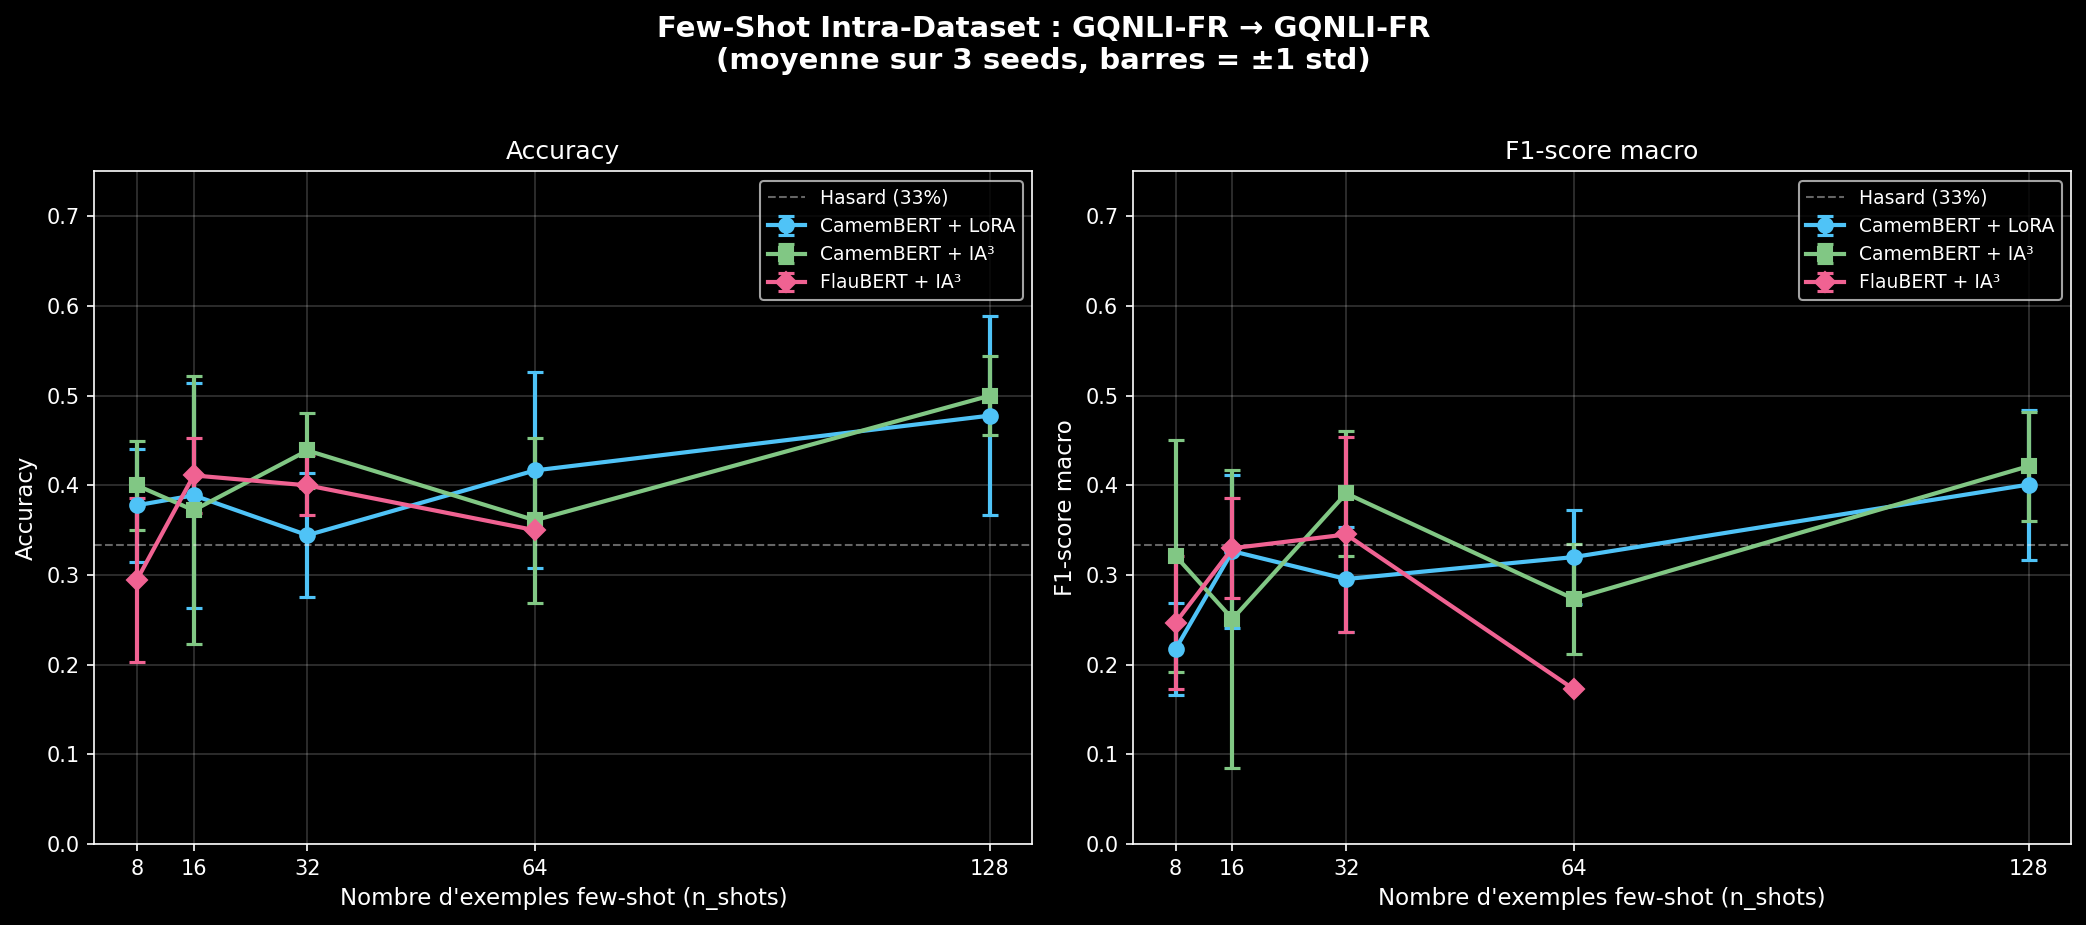
\includegraphics[width=0.9\textwidth]{results/metricsgraphs/few_shot_intra_gqnli.png}
    \caption{Évolution de l'accuracy et du Score F1 (Macro) en fonction du nombre de "shots".}
    \label{fig:intra}
\end{figure}

Comme l'illustre la figure \ref{fig:intra}, **l'approche IA$^3$ obtient la victoire absolue sur le segment Extreme Few-Shot.**
Dès le palier de 8 exemples, \texttt{CamemBERT + IA$^3$} atteint \textbf{40.0\%} d'accuracy (battant le hasard) tandis que \texttt{CamemBERT + LoRA} stagne sous les 38\%. Sur le plafond des 128 exemples, IA$^3$ maintient son avance en perçant la barre des \textbf{50.0\%}. La "légèreté" paramétrique de l'IA$^3$ empêche le modèle de mémoriser mécaniquement le bruit des 8 phrases, favorisant une abstraction de la tâche et confirmant la supériorité de cette méthode pour des corpus pauvres.

\section{Résultats 2 : Le Cross-Dataset (Transfert de Domaine)}
L'expérience finale (\textit{Sweep t493ddfp}) cherchait à forcer le modèle à généraliser. Nous lui avons fourni des axiomes de logique formelle mathématiques (dataset \textbf{FraCaS}) et l'avons testé sur des descriptions d'articles Wikipédia (\textbf{GQNLI-FR}).

\begin{figure}[h!]
    \centering
    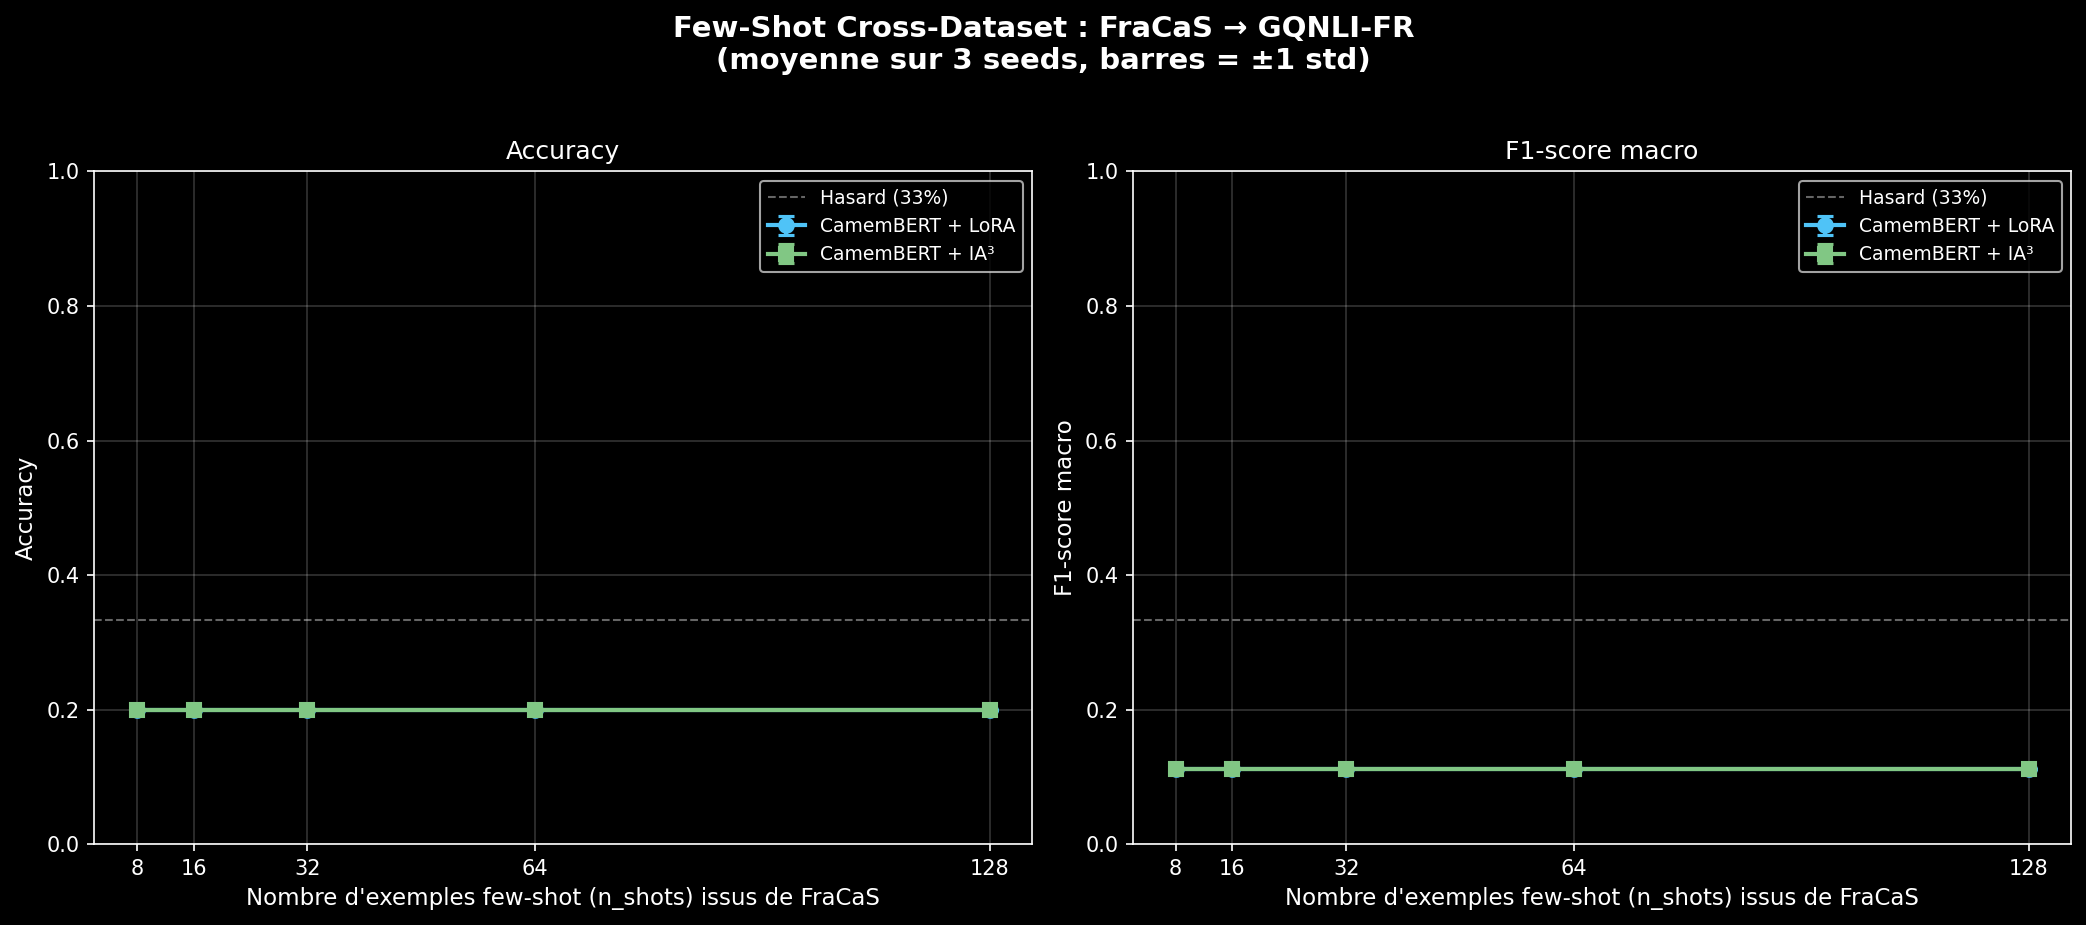
\includegraphics[width=0.9\textwidth]{results/metricsgraphs/few_shot_cross_fracas_gqnli.png}
    \caption{Effondrement catastrophique en transfert Cross-Dataset (FraCaS vers GQNLI).}
    \label{fig:cross}
\end{figure}

Les résultats dévoilent un mécanisme fascinant du NLI profond : \textbf{une chute immuable à 20.0\%} d'exactitude (pire que le hasard de 33\%, pré-disant la classe "Neutre" pour l'intégralité du set de test).
Durant le Fine-Tuning, le modèle a instantanément percé la structure rigide de FraCaS (atteignant une validation de $100\%$). Néanmoins, s'agissant de pur "Few-Shot", cette logique mathématique agit comme un format parasite qui détruit la capacité naturelle de compréhension sémantique de GQNLI. C'est la limite ultime démontrée : en Few-Shot, le transfert interdisciplinaire est un échec par défaut.

\section{Conclusion}
Au terme de ces sweeps complets, nous avons scientifiquement cartographié les limites de l'usage NLI. Le plein-potentiel réside dans le Full-Data ($\sim 80\%$), mais si les budgets ne le permettent pas, une fine couche de restriction IA$^3$ permet néanmoins d'extirper la moitié des bonnes réponses possibles ($\sim 50\%$) avec des requêtes rudimentaires, à condition absolue d'opérer le modèle dans son strict domaine d'apprentissage lexical.

\end{document}
